\documentclass[a4paper,12pt, english]{article}
\usepackage[T1]{fontenc}
\usepackage[utf8]{inputenc}
\usepackage{graphicx}
\usepackage{babel}
\usepackage{amsmath}
\usepackage{ulem}
\usepackage{a4wide}
\usepackage{graphicx}
\usepackage{listings}
\usepackage{tabularx}
\usepackage{tabulary}

\begin{document}

\section*{Project 1}
In this project we want to solve the boundary value equation $ -u''(x) = f(x) $ with $ x \hspace{1mm} \epsilon \hspace{1mm}  (0,1) $ and boundary conditions $ u(0) = u(1) = 0 $. This is the one-dimensional Poisson equation with Dirichlet boundary conditions.
Our original differential equation can be written as a discretized equation where we approximate the second derivative of u with $$ - \frac{v_{i+1}+v_{i-1}-2v_{i}}{h^2} = f_{i} $$ 
for $ i = 1, ..., n $ and $ v_{0} = v_{n+1} = 0$.

Our goal in this project is to rewrite this equation to a set of linear equations and solve the approximation both analytical and numerical. 

\begin{enumerate}
\item[(a)]
We can rewrite the differential equation as a system of linear equations $$ Av = \tilde{b}. $$
With
\[ A = \left( \begin{array}{cccccc}
2 & -1 & 0 & ... & ... & 0\\
-1 & 2 & -1 & 0 & ... & ... \\
0 & -1 & 2 & -1 & 0 & ... \\
... & ... & ... & ... & ... &...\\
0 & ... & ... & -1 & 2 & -1 \\
0 & ... & ... & 0 & -1 & 2 \end{array} \right)\] 
and the vectors
\[ v = \left( \begin{array}{c}
v_{1}\\
v_{2}\\
...\\
...\\
...\\
v_{n} \end{array} \right)\]  

\[ \tilde{b} = \left( \begin{array}{c}
\tilde{b_{1}}\\
\tilde{b_{2}}\\
...\\
...\\
...\\
\tilde{b_{n}} \end{array} \right)\]

 Here $v_{i}$ are the unknowns in the second derivative approximation and $\tilde{b_{i}} = h^2 f_{i} $.
We see that our system then reproduce the equations for the approximation of the second derivative.

Matrix multiplication produce the linear equations:
$$2v_{1} - v_{2} = \tilde{b_{1}} \hspace{10mm} (1)$$
$$-v_{1} +2v_{2} - v_{3} = \tilde{b_{2}} \hspace{10mm} (2)$$
$$ ... $$
From the approximation of u:

For i = 1: $$ -\frac{v_{2}+v_{0}-2v_{1}}{h^2} = f_{1} $$ where $v_{0}=0$.
$$-v_{2}+2v_{1} = h^2 f_{1} = \tilde{b_{1}} \hspace{10mm} (1)$$
For i = 2: $$ -\frac{v_{3}+v_{1}-2v_{3}}{h^2} = f_{2} $$
$$-v_{1} +2v_{2} - v_{3} = h^2f_{2} = \tilde{b_{2}} \hspace{10mm} (2)$$
$$...$$

We assume that the source term is $f(x) = 100 e^{-10x}$ and keep the same interval and boundary equations.

The differential equation has an analytical solution given by $$u(x) = 1 - (1-e^{-10})x - e^{10x}. $$
Since
$$u'(x) = -1 + e^{-10} + 10e^{-10x} $$
$$u''(x) = -100e^{-10x} = - f(x)$$
we see that this solution is in agreement with Poisson's equation.

\item[(b)] 
We can use the linear equation derived in subproblem (a), $Av = \tilde{b}$, to solve the Poisson equation numerically. 

The matrix $A$ is a tridiagional matrix, with non-zero elements only in the main diagonal and those immediately above and below. In our case all the elements in the three diagonals respectively have the same value. 

In my program I read the size of the matrix $n$ from the command line. Thereafter I allocate arrays of that size for the three non-zero diagonals, the unknowns $v_{i}$ and the function values $\tilde{b_{i}}$.

I use forward substitution to eliminate all the elements in the lower diagonal. Thereafter I use backward substitution to do the same to the upper diagonal elements. We are then left with n equations with the 		unknowns $v_{i} = \frac{\tilde{b_{i}}}{b_{i}}$.

I then feed the solutions $v_{i}$ and the $n$-value into a file, and use a python script to make a plot of the derived solution together with the analytical solution. To get the right boundaries I only feed the inner values of $v$ to the file. In the python script I give the first and last value, which is given by the boundary conditions to be zero. 


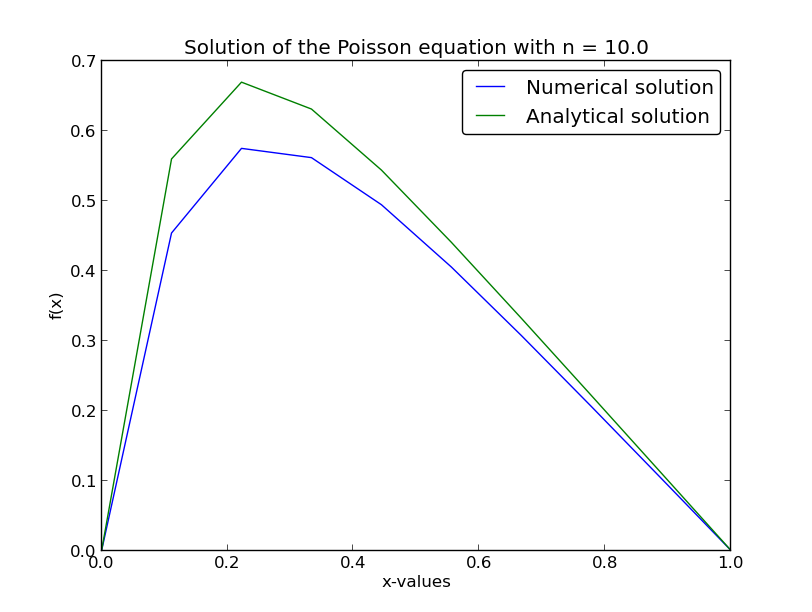
\includegraphics[scale=0.5]{opgb_n10} 
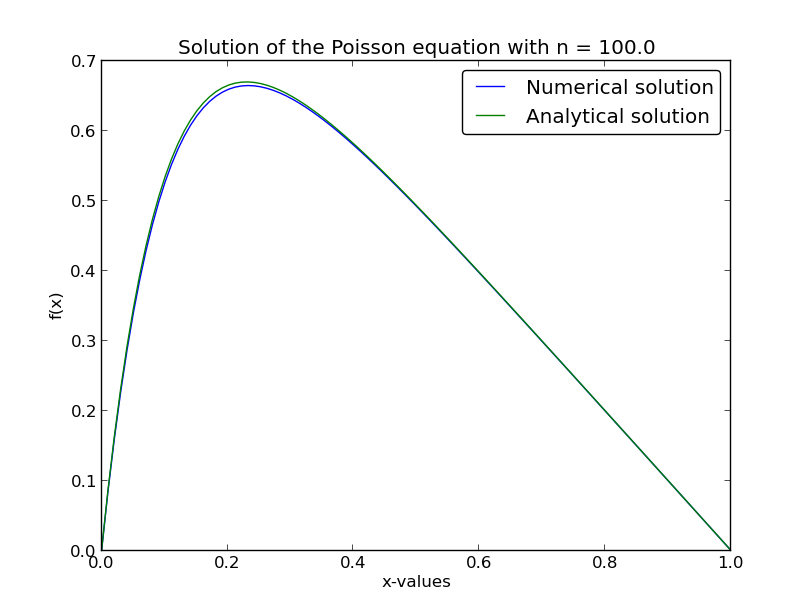
\includegraphics[scale=0.5]{opgb_n100} 
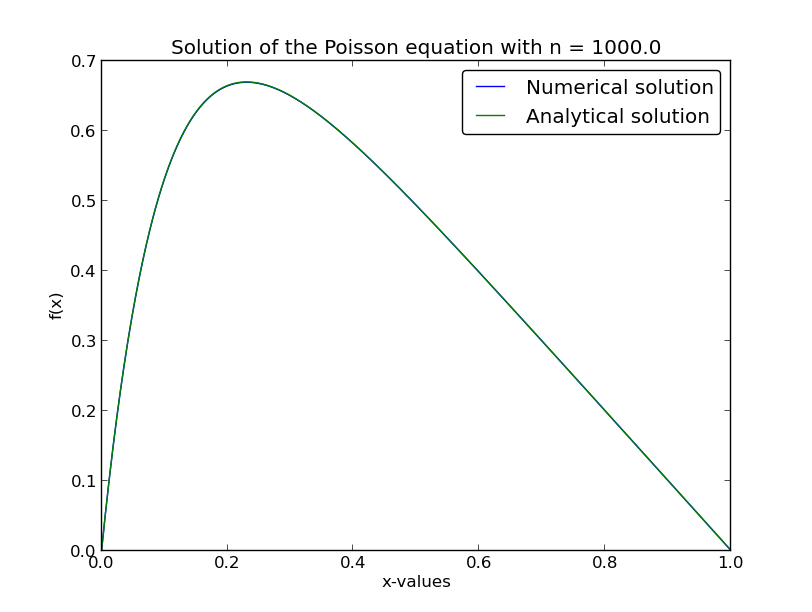
\includegraphics[scale=0.5]{opgb_n1000} 

To find the number of flops used in the forward and backward substitution we can count the number of operations used in the program.   

\begin{lstlisting}[title={Code abstract}]
// forward substitution

    for (i=1; i<n-1; i++) {
        b[i+1] = b[i+1] - (a[i+1]/b[i])*c[i];
        b_tilde[i+1] = b_tilde[i+1] - (a[i+1]/b[i])*b_tilde[i];

    }

    // backward substitution

    v[n-2] = b_tilde[n-2] / b[n-2];
    for (i=n-2; i>0; i--){
        v[i-1] = (b_tilde[i-1] - c[i]*v[i]) / b[i-1];
    }
\end{lstlisting}

In the forward substitution I have one subtraction, multiplication and division for both the calculation of $b_{i}$ and $\tilde{b_{i}}$. These six floating point operations are performed $n-2$ times. Number of flops in the forward substitution therefore goes as $6n$. 

In the backward substitution we have three floating point operations, subtraction, multiplication and division as before. The number of flops for the backward substitution goes as $3n$. 

We then have a total floating point operations per second $6n+3n = 9n \sim O(n)$.

Our method for solving the equation with the tridigonal matrix has proven to be an efficient one. Gaussian elimination requires many more floating operations. When using the Gaussian method one does not take into account the many zero elements, and unnecessary many operations are being made for these elements. When using Gaussian elimination a $nxn$ matrix requires $\frac{2n^3}{3} + O(n^2)$ floating point operations. 
Our algorithm runs faster than a LU decomposition as well. An LU decomposed matrix requires $O(n^2)$ flops. In addition one will need roughly $O(n^3)$ flops to obtain the LU decomposed matrix. 
 
\item[(c)]
To find the relative error for different step lengths I iterate over different $n$-values. For each value I compile and run my c++ program to extract the correct $v_{i}$ and $u_{i}$ values. I then take the base ten logarithm of the absolute value of the difference between the analytical and numerical solution. 

\[
 \epsilon_i=log_{10}\left(\left|\frac{v_i-u_i}
                 {u_i}\right|\right),
\]

Thereafter I pick out the maximum value of the relative error, and use this point when plotting against the logarithm of the corresponding $h$-value. I vary $n$ from $10$ to $10^5$.  

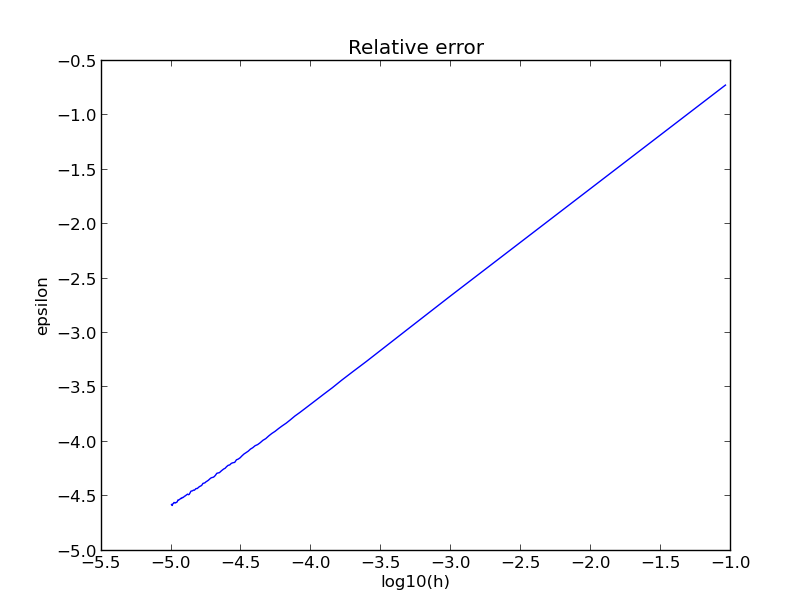
\includegraphics[scale=0.5]{opgc}

When plotting the relative error we see that the error reduces linearly. For big $n$-values however, the line fluctuates somewhat. This could be evidence that our program is more unstable for large $n$, that is $n \sim 10^5$. 


\item[(d)]
The task in this subproblem is to compare the results with those from LU decomposition. To do this I first set up the tridiagonal matrix $A$  and the vector $\tilde{b}$. Then I used the LU-decomposition from the armadillo library to calculate the lower and upper matrices L and U. The matrix $A$ can then be written as the product of the two matrices L and U. $$ Av = \tilde{b}$$ $$Av = LUv = \tilde{b}$$
In my program I calculate this in two steps $$Lx = \tilde{b} \hspace*{15mm} Uv = x $$
After using the known values of $L$ and $\tilde{b}$ to calculate $x$, I use $x$ and $U$ to calculate the desired $v$-values.
I compute the elapsed time needed to do the LU-decomposition and to find the $v$-values through matrix multiplication. I take the time used in my tridiagonal solver as well, to compare the difference in time needed. 

\begin{center}
\begin{tabular}{l | c | c}

n-values & Time needed for LU decomposition (sec) & Time needed for tridiagonal solver (sec) \\ \hline 
10 & 0 & 0 \\ 
100 & 0.01 & 0 \\
1000 & 0.33 & 0 \\
\end{tabular}
\end{center}

We see that for the tridiagonal solver our program runs fast for all the tested $n$-values. The time needed to perform the LU decomposition however, increases quite a lot as $n$ increases. 

To obtain the LU decomposed matrix one uses $O(n^3)$ floating point operations. So it is no wonder that the time needed to do the LU decomposition increases more drastically with $n$ than our tridiagonal solver that uses $O(n)$ flops. After having calculated the upper and lower matrices, only two multiplications is needed to find the $v_{i}$-values. When trying to run the program for a $10^5 x 10^5$ matrix I get an error code telling me that the requested size is to large. Evidently my machine has not got enough memory to do the LU calculations for a matrix this size. 

\item[(e)]
The aim her is to test possible memory strides when performing operations on matrices. First I initialize the matrices $B$ and $C$, and compute the multiplication $A = BC$. Then I compute the time needed for the matrix multiplications.

\begin{center}
\begin{tabular}{l | c}
n-values & Time needed for matrix multiplication (sec) \\ \hline 
10 & 0\\ 
100 & 0.04\\
1000 & 47.54 \\
\end{tabular}
\end{center}
\end{enumerate}


We see that for $n=1000$ the time needed increases dramatically. For a matrix of dimension $10^4$, as requested in the text, my program uses so long time that I have not got patience to wait for the result. Thus we see that matrix multiplication is a time consuming operation. 

\subsubsection*{List of codes}
\begin{center}
\begin{tabular}{l  c}
main.cpp & subproblem b \\
LU.cpp & subproblem d \\
matrix\_operations.cpp &  subroblem e \\
plot.py & subproblem b and c \\
\end{tabular}
\end{center}

\end{document}